\section{Algorithm}

\subsection{Overview}

For both the 2D and 3D generalized Hilbert (Gilbert) curve, a template is chosen
to recursively subdivide the area or volume.
When recursively descending the sub-volumes, we will need to translate to
a new reference point and rotate by increments of $(\pi/2)$ radians, maintaining
cuboid regions that are axis-aligned.
We use the convention of labeling $\alpha, \beta, \gamma \in \mathbb{Z}^3$ for
the width-like, height-like and depth-like dimension vectors, respectively.

Each of $\alpha$, $\beta$ and $\gamma$ start off as axis-aligned vectors of integral
length and are only rotated by units of $(\pi/2)$ radians, remaining axis aligned throughout.
$\alpha$, $\beta$ and $\gamma$ represent the dimensions of the sub-cuboid region
and the local basis when tracing out a curve.

The next sub-section discusses parity arguments for when a valid curve can be
traced out in a sub-region.
We then discuss the 2D Gilbert curve and end with the 3D Gilbert curve.

When talking about the 2D Gilbert curves, we assume vectors are in $\mathbb{Z}^3$
so they can be used without alteration for algorithms working in 3D.

%In what follows, a path is assumed to start at the local reference point $(0,0,0)$
%and end at the far edge of the the width like dimension, $\alpha$ (e.g. $(w-1,0,0)$).

\subsection{Valid Paths from Grid Parity}

\begin{figure}[h]
  \centering
  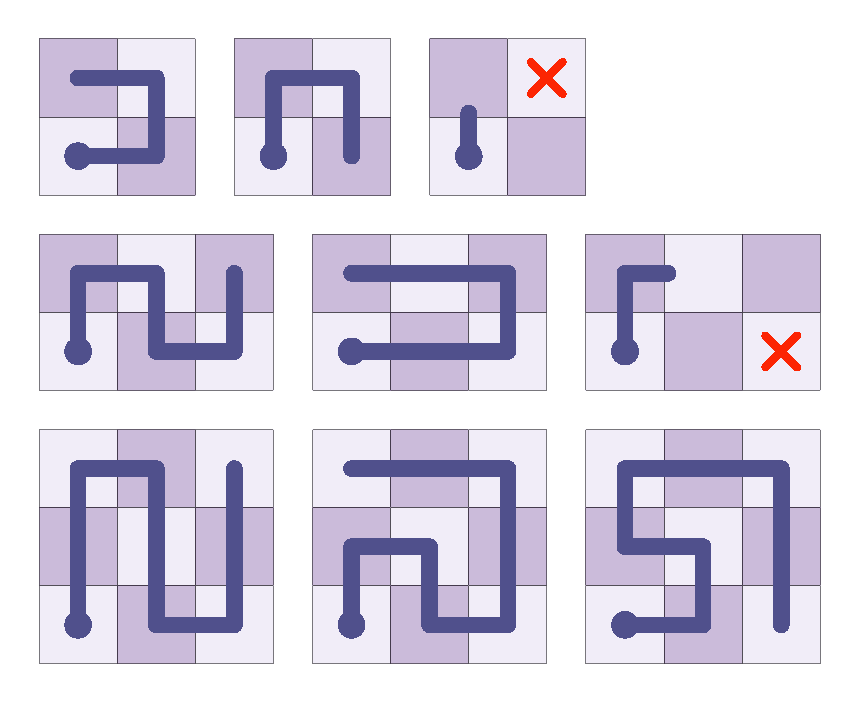
\includegraphics[width=\linewidth]{simple_hampath.pdf}
  \caption{ Illustrative examples of Hamiltonian paths height/width that are even/even, even/odd and odd/odd, respectively,
            when starting from the lower left hand corner }
  \label{fig:exampleHampath}
\end{figure}


The feasibility of determining whether there exists a Hamiltonian path in a rectangular cuboid
grid region can be accomplished through parity arguments.
Label grid cell points in a volume as 0 or 1,
alternating between labels with every axis-aligned single step move.
Any Hamiltonian path that ends at one of the three remaining corners has to have the same parity as the starting point if the
volume is odd, or different parity if the volume is even.

\begin{table}[h]
  \centering
  \begin{tabular}[t]{cr|cc}
    \multicolumn{2}{c}{ \multirow{2}{*}{Path Possible} } & \multicolumn{2}{c}{Volume} \\
    & & \textit{even} & \textit{odd} \\
    \hline
			%\multirow{2}{*}{$|\alpha| \bmod 2$} & \textit{even} & Yes & Yes \\
      \multirow{2}{*}{ $|\alpha|$ } & \textit{even} & Yes & Yes \\
       & \textit{odd} & \textbf{No} & Yes \\
     \hline
  \end{tabular}
  \caption{ Table showing when a Hamiltonian cycle is possible. Here, $|\alpha|$ is the absolute difference in start and end position of the path which
            coincides with one of the axis aligned side length of the cuboid volume. A Hamiltonian path is not possible on only in the case
            when $|\alpha|$ is odd and the volume is even. }
  \label{table:pathTable}
\end{table}


For a path starting at $(0,0,0)$ and ending $|\alpha|$ steps in one of the axis-aligned dimensions,
then Table \ref{table:pathTable} enumerates this condition under which a valid path is possible.
Figure \ref{fig:exampleHampath} illustrates this for starting position $(0,0)$ with volumes $(2 \times 2)$, $(3 \times 2)$ and $(3 \times 3)$,
where a red cross indicating a precluded endpoint.

Without loss of generality, we will assume a curve starts from position $p_s=(0,0,0)$ and has proposed
endpoint at $p_e=((w-1),0,0)$, with a cuboid region as $\alpha = (w,0,0), \beta = (0,h,0), \gamma = (0,0,d)$.
We state, without proof, that
a Hamiltonian path is always possible from $p_s$ to $p_e$ when $|\alpha|$ is even or when $|\alpha|$, $|\beta|$ and $|\gamma|$
are all odd  $(|\alpha| \cdot (1 - |\beta| \cdot |\gamma|) \equiv 0 \bmod 2)$.

With this condition, any cuboid subdivision will always have a Hamiltonian path within it and we can recreate a Hamiltonian
path in the larger cuboid by connecting endpoints from the ending point of one cuboid to the starting point of the succeeding cuboid.
For cuboids that violate this condition, there will be a required notch and we will show that an admissible cuboid subdivision is possible
for all but one of the cuboid subdivisions, recursively limiting the notch violation to a single point.


%%%%%%%%%%%%%%%%%%%%%%%%%%%%%%%%%%%%%%%%%%%%%%%%
%            _ ____              __ ___       __
%     ____ _(_) / /_  ___  _____/ /|__ \ ____/ /
%    / __ `/ / / __ \/ _ \/ ___/ __/_/ // __  / 
%   / /_/ / / / /_/ /  __/ /  / /_/ __// /_/ /  
%   \__, /_/_/_.___/\___/_/   \__/____/\__,_/   
%  /____/                                       
%%%%%%%%%%%%%%%%%%%%%%%%%%%%%%%%%%%%%%%%%%%%%%%%


\subsection{2D Generalized Hilbert Function (Gilbert2D)}

\begin{figure}[h]
  \centering
  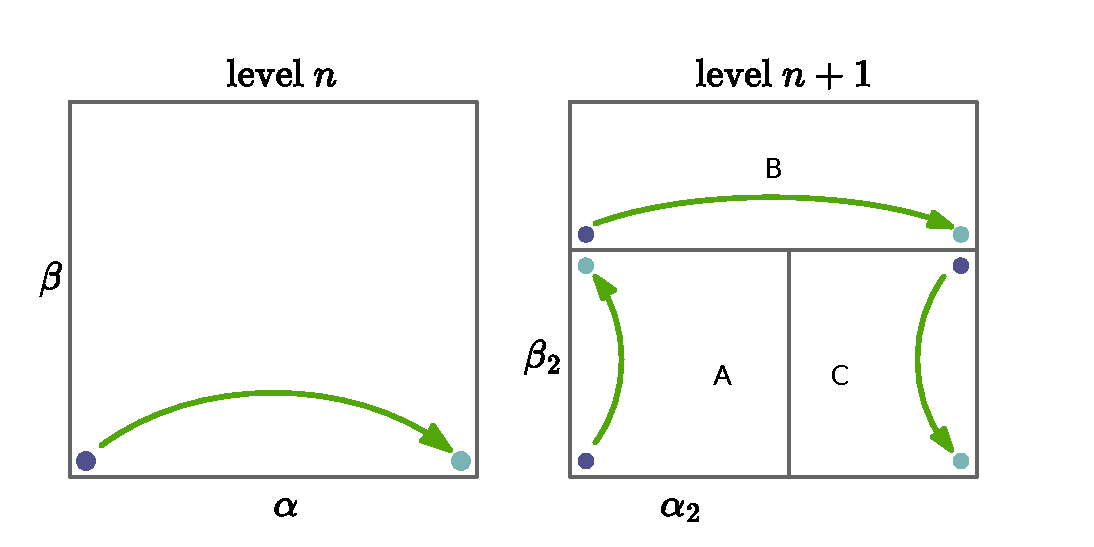
\includegraphics[width=\linewidth]{gilbert2d_mainsubdiv.pdf}
  \caption{ For the 2D Gilbert curve, the main rectangle is subdivided into three sub regions, making sure their paths connect
            and preferring even side lengths for the first rectangular subdivision.
            Partitioning the rectangle in this way is what we call a $U$-split.  }
  \label{fig:main2dsubdiv}
\end{figure}


\begin{figure*}[ht]
  \centering
  \includegraphics[width=\linewidth]{config_production.pdf}
  \caption{ Enumeration of the subdivision template depending on different parities of $\alpha$ and $\beta$ dimensions. }
  \label{fig:production2d}
\end{figure*}

For the 2D Gilbert curve, a $U$-split template is used, highlighted in figure \ref{fig:main2dsubdiv}.
The $U$-split breaks the region into three sub-blocks, labeled $A$, $B$ and $C$.
Each of the $A$, $B$ and $C$ regions have local coordinate systems that are resized, rotated and
new endpoints chosen so the process can be recursively re-applied.

The sides of the subdivided blocks $A$, $B$ and $C$ are chosen to remain integral.
The width-like dimension for subdivided block $A$ is chosen to be even ($\beta_2$ in Figure \ref{fig:main2dsubdiv})
by dividing the width-like dimension by two and by adding one if need be.
Since the width-like length of the subdivided $A$ and $C$ block is even, there is still a valid Hamiltonian path 
in both.

Should the original width-like be even ($\alpha$ in \ref{fig:main2subdiv}), the $C$ block will continue to have 
a valid Hamiltonian path.
If the original width-like dimension is odd, there is a forced notch that will appear in the subdivided block $C$.

Figure \ref{fig:production2d} gives examples of the different parity conditions for the original area,
as well as the different conditions when the $A$ and $C$ subdivided areas are force even parity.
Figure \ref{fig:production2d} also shows when a Hamiltonian
path is not possible, indicated by a red cross, and illustrates how the notch is pushed into the $C$ block
under these conditions.

If a subdivided block becomes too long in its width-like dimension, the block is divided in half and the recursion
proceeds as normal.
Even sides are only enforced if the length is larger than 2, with a length 2 or smaller representing the base
case.
The base case enumerates paths in the non trivial direction.

Since $A$ and $C$ are chosen to have an even width-like local axis length, no new notches are introduced and any
obligatory notch is effectively ``pushed'' into the $C$ block.


%The $A$ block is chosen to to have a preference for even height dimension


\begin{algorithm}
  \caption{\hskip0.5em 2D Generalized Hilbert Function (Gilbert2D) } %($p$, $\alpha$, $\beta$) \\ \hskip3.0em $p, \alpha, \beta \in \mathbb{Z}^3$ }
  \label{alg:gilbert2d}
  \begin{algorithmic}

    \State \textit{\# $p, \alpha, \beta \in \mathbb{Z}^3$}
    \Function{Gilbert2D}{$p$, $\alpha$, $\beta$}
      \State
      \State $\alpha_2, \beta_2  = (\alpha // 2), (\beta // 2)$

      \State
      \If{ $(|\beta| \equiv 1)$ }
        \State \textbf{yield} $p + i \cdot \delta(\alpha)$ \textbf{forall} $i \in |\alpha|$

        \State
      \ElsIf{ $(|\alpha| \equiv 1)$ }
        \State \textbf{yield} $p + i \cdot \delta(\alpha)$ \textbf{forall} $i \in |\beta|$

        \State
      \ElsIf{ $(2 |\alpha| > 3 |\beta|)$ }
        \If{ $(|\alpha_2| > 2)$ and $(|\alpha_2| \bmod{2} \equiv 1)$ }
          \State $\alpha_2 \leftarrow \alpha_2 + \delta(\alpha)$
        \EndIf
        \State
        \State \textbf{yield} Gilbert2D($p$, \\ \hskip9.75em $\alpha_2$, $\beta$)
        \State
        \State \textbf{yield} Gilbert2D($p + \alpha_2$, \\ \hskip9.75em $\alpha - \alpha_2$, $\beta$)

        \State
      \Else
        \If{ $(|\beta_2| > 2)$ and $(|\beta_2| \bmod{2} \equiv 1)$ }
          \State $\beta_2 \leftarrow \beta_2 + \delta(\beta)$
        \EndIf
        \State
        \State \textbf{yield} Gilbert2D($p$, \\ \hskip9.75em $\beta_2$, $\alpha_2$)
        \State
        \State \textbf{yield} Gilbert2D($p + \beta_2$, \\ \hskip9.75em $\alpha$, $(\beta - \beta_2)$)
        \State
        \State \textbf{yield} Gilbert2D($p + \alpha - \delta(\alpha) + \beta_2 - \delta(\beta)$, \\ \hskip9.75em $\beta_2$, $-(\alpha - \alpha_2)$)
      \EndIf
    \EndFunction
  \end{algorithmic}
\end{algorithm}

Algorithm \ref{alg:gilbert2d} shows the pseudo-code for computing the 2D Gilbert curve.
Note that $\alpha$ and $\beta$ are taken to be vectors in 3D, where the third dimension
can be ignored if a purely 2D curve is desired.
The generalization to 3D allows the Gilbert2D function to be used unaltered when the
3D Gilbert curve needs to trace out in-plane sub-curves.

\floatname{algorithm}{Procedure}
\begin{algorithm}
  \caption{\hskip0.5em $\delta(\cdot)$ directional vector function }
  \label{alg:delta}
  \begin{algorithmic}

    \State
    \State \textit{\# integral sign function}
    \Function{$\text{sgn}$}{$w \in \mathbb{Z}$}
      %\State $(w < 0) ? (-1) : ((w > 0) ? 1 : 0)$
      \State \textbf{if} $(w < 0)$ \Return $-1$
      \State \textbf{if} $(w > 0)$ \Return $1$
      \State \Return 0
    \EndFunction

    \State
    \State \textit{\# directional vector}
    \Function{$\delta$}{$v \in \mathbb{Z}^3$}
      \State \Return $[ \text{sgn}(v_0), \text{sgn}(v_1), \text{sgn}(v_2) ]$
    \EndFunction

  \end{algorithmic}
\end{algorithm}
\floatname{algorithm}{Algorithm}

The $\delta(\cdot)$ function returns one of the six directional vectors indicating which of
the major signed axis aligned directions the input vector points to ($[\pm1,0,0], [0,\pm1,0],[0,0,\pm1]$).
For completeness, the function is defined in Procedure \ref{alg:delta}.

Algorithm \ref{alg:gilbert2d} assumes standard Euclidean two norm ($|v| = \sqrt{v_0^2 + v_1^2 + v_2^2}$)
and abuses notation by allowing scalar to vector multiplication ($i \in \mathbb{Z}, v \in \mathbb{Z}^3, i \cdot v \to [ i \cdot v_0, i \cdot v_1, i \cdot v_2 ]$).
where the context is clear.

Example outputs of the \textit{Gilbert2D} function are listed in Figure \ref{fig:gilbert2d_examples}, showing a $(4 \times 4)$, $(10 \times 4)$ and $(7 \times 4)$

%%%%%%%%%%%%%%%%%%%%%%%%%%%%%%%%%%%%%%%%%%%%%%%%%
%            _ ____              __ _____     __
%     ____ _(_) / /_  ___  _____/ /|__  /____/ /
%    / __ `/ / / __ \/ _ \/ ___/ __//_ </ __  / 
%   / /_/ / / / /_/ /  __/ /  / /____/ / /_/ /  
%   \__, /_/_/_.___/\___/_/   \__/____/\__,_/   
%  /____/                             
%%%%%%%%%%%%%%%%%%%%%%%%%%%%%%%%%%%%%%%%%%%%%%%%%

\subsection{3D Generalized Hilbert Function (Gilbert3D)}

\begin{figure}[h]
  \centering
  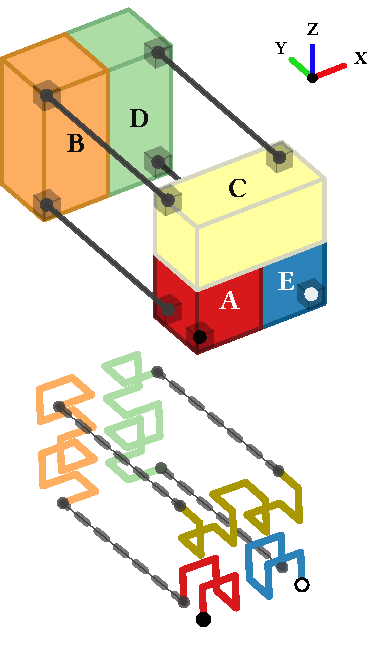
\includegraphics[width=\linewidth]{gilbert3d_explode.pdf}
  \caption{ The $J_0$-split subdivision, representing the main subdivision of the bulk recursion for the 3D Gilbert curve case. }
  \label{fig:gilbert3DJSplit}
\end{figure}


The concept of a $U$-split is extended into 3D by constructing a $J$-split.
An exploded view of a $J$-split is showing in Figure \ref{fig:gilbert3DJSplit}.

Side lengths of the subdivided cuboids are chosen to try and not preclude a
Hamiltonian path.
If a path starts at the local $[0,0,0]$, a Hamiltonian path that ends
at $[(w-1),0,0]$ is only possible when $w$ is even or when all lengths are odd, including $w$.


\begin{figure*}[ht]
  \centering
  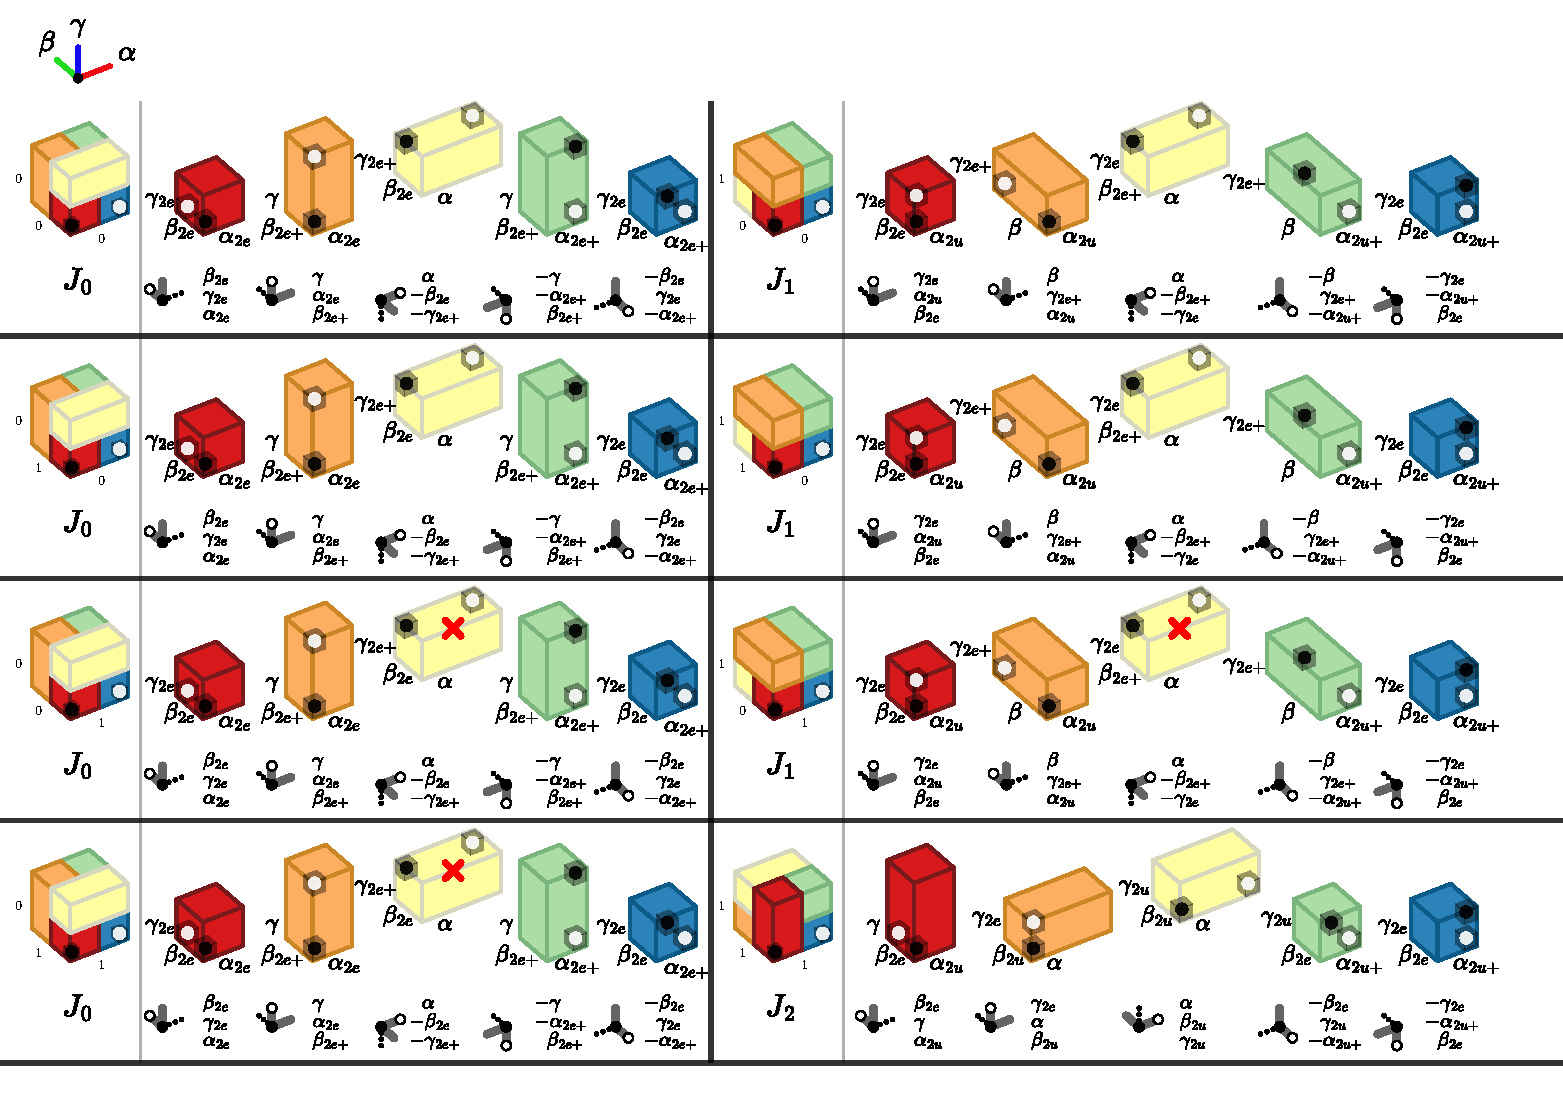
\includegraphics[width=\textwidth]{gilbert3d_case.pdf}
  \caption{ Bulk recursion J-split atlas for the 3D Gilbert algorithm }
  \label{fig:gilbert3DCase}
\end{figure*}

\floatname{algorithm}{Procedure}
\begin{algorithm}
  \caption{ \hskip0.5em $S_0$-Split function (eccentric split) }
  \label{alg:procS0}
  \begin{algorithmic}
    \State
    \State \textit{\# split halfway on $\alpha$ }
    \Function{$S_0$}{$p$, $\alpha$, $\beta$, $\gamma$}
      \State $\alpha_2 \leftarrow (\alpha // 2)$
      \If{ $(|\alpha| > 2)$ and $((|\alpha_2| \bmod{2}) \equiv 1)$ }
        \State $\alpha_2 \leftarrow \alpha_2 + \delta(\alpha)$
      \EndIf
      \State
      \State \textbf{yield} Gilbert3D($p$, \\ \hskip8.25em $\alpha_{2}$, $\beta$, $\gamma$ )
      \State
      \State \textbf{yield} Gilbert3D($p + \alpha_{2}$, \\ \hskip8.25em $(\alpha - \alpha_{2})$, $\beta$, $\gamma$ )
    \EndFunction
  \end{algorithmic}
\end{algorithm}
\floatname{algorithm}{Algorithm}


\floatname{algorithm}{Procedure}
\begin{algorithm}
  \caption{ \hskip0.5em $S_1$-Split functions (eccentric split) }
  \label{alg:procS1}
  \begin{algorithmic}
    \State
    \State \textit{\# split $\frac{1}{3}$ on $\gamma$ and halfway on $\alpha$ }
    \Function{$S_1$}{$p$, $\alpha$, $\beta$, $\gamma$}
      \State $\alpha_2, \gamma_3 \leftarrow (\alpha // 2), (\gamma // 3)$
      \If{ $(|\alpha| > 2)$ and $((|\alpha_2| \bmod{2}) \equiv 1)$ }
        \State $\alpha_2 \leftarrow \alpha_2 + \delta(\alpha)$
      \EndIf
      \If{ $(|\gamma| > 2)$ and $((|\gamma_3| \bmod{2}) \equiv 1)$ }
        \State $\gamma_3 \leftarrow \gamma_3 + \delta(\gamma)$
      \EndIf
      \State
      \State \textbf{yield} Gilbert3D($p$, \\ \hskip8.25em $\gamma_3$, $\alpha_2$, $\beta$)
      \State
      \State \textbf{yield} Gilbert3D($p + \gamma_3$, \\ \hskip8.25em $\alpha$, $\beta$, $(\gamma - \gamma_3)$)
      \State
      \State \textbf{yield} Gilbert3D($p + \alpha - \delta(\alpha) + \gamma_{3} - \delta(\gamma)$, \\ \hskip8.25em $\gamma_3$, $(\alpha - \alpha_2)$, $\beta$)
    \EndFunction
  \end{algorithmic}
\end{algorithm}
\floatname{algorithm}{Algorithm}


\floatname{algorithm}{Procedure}
\begin{algorithm}
  \caption{ \hskip0.5em $S_2$-Split function (eccentric split) }
  \label{alg:procS2}
  \begin{algorithmic}
    \State
    \State \textit{\# split $\frac{1}{3}$ on $\beta$ and halfway on $\alpha$ }
    \Function{$S_2$}{$p$, $\alpha$, $\beta$, $\gamma$}
      \State $\alpha_2, \beta_3 \leftarrow (\alpha // 2), (\beta // 3)$
      \If{ $(|\alpha| > 2)$ and $((|\alpha_2| \bmod{2}) \equiv 1)$ }
        \State $\alpha_2 \leftarrow \alpha_2 + \delta(\alpha)$
      \EndIf
      \If{ $(|\beta| > 2)$ and $((|\beta_3| \bmod{2}) \equiv 1)$ }
        \State $\beta_3 \leftarrow \beta_3 + \delta(\beta)$
      \EndIf
      \State
      \State \textbf{yield} Gilbert3D($p$, \\ \hskip8.25em $\beta_{3}$, $\gamma$, $\alpha_2$ )
      \State
      \State \textbf{yield} Gilbert3D($p + \beta_{3}$, \\ \hskip8.25em $\alpha$, $(\beta - \beta_{3})$, $\gamma$ )
      \State
      \State \textbf{yield} Gilbert3D($p + \alpha - \delta(\alpha) + \beta_{3} - \delta(\beta)$, \\ \hskip8.25em $-\beta_{3}$, $\gamma$, $-\alpha$)
    \EndFunction
  \end{algorithmic}
\end{algorithm}
\floatname{algorithm}{Algorithm}


\floatname{algorithm}{Procedure}
\begin{algorithm}
  \caption{ \hskip0.5em $J_0$-Split function }
  \label{alg:procJ0}
  \begin{algorithmic}
    \State
    \State \textit{\# $|\gamma|$ even }
    \Function{$J_0$}{$p$, $\alpha$, $\beta$, $\gamma$}
      \State
      \State $\alpha_2, \beta_2, \gamma_2 \leftarrow (\alpha // 2), (\beta // 2), (\gamma // 2)$
      \State
      \State \textit{\# prefer initial block even}
      \State $\alpha_2=\alpha_2+\delta(\alpha)$ \textbf{if} $(|\alpha_2| > 2)$and$(|\alpha_2| \bmod{2} \equiv 1)$
      \State $\beta_2=\beta_2+\delta(\beta)$ \textbf{if} $(|\beta_2| > 2)$and$(|\beta_2| \bmod{2} \equiv 1)$
      \State $\gamma_2=\gamma_2+\delta(\gamma)$ \textbf{if} $(|\gamma_2| > 2)$and$(|\gamma_2| \bmod{2} \equiv 1)$
      \State
      \State \textbf{yield} Gilbert3D($p$, \\ \hskip8.25em $\beta_2$, $\gamma_2$, $\alpha_2$)
      \State
      \State \textbf{yield} Gilbert3D($p+\beta_2$, \\ \hskip8.25em $\gamma$, $\alpha_2$, $\beta - \beta_2$)
      \State
      \State \textbf{yield} Gilbert3D($p + \beta_2 - \delta(\beta_2) + \gamma - \delta(\gamma)$, \\ \hskip8.25em $\alpha$, $-\beta_2$, $-(\gamma - \gamma_2)$)
      \State
      \State \textbf{yield} Gilbert3D($p + \alpha - \delta(\alpha) + \beta_2 + \gamma - \delta(\gamma)$, \\ \hskip8.25em $-\gamma$, $-(\alpha - \alpha_2)$, $(\beta - \beta_2)$)
      \State
      \State \textbf{yield} Gilbert3D($p + \alpha - \delta(\alpha) + \beta_2 - \delta(\beta)$, \\ \hskip8.25em $-\beta_2$, $\gamma_2$, $-(\alpha - \alpha_2)$)
    \EndFunction
  \end{algorithmic}
\end{algorithm}
\floatname{algorithm}{Algorithm}


\floatname{algorithm}{Procedure}
\begin{algorithm}
  \caption{ \hskip0.5em $J_1$-Split function }
  \label{alg:procJ2}
  \begin{algorithmic}
    \State
    \State \textit{\# $|\gamma|$ odd, one of $|\alpha|$ or $|\beta|$ even }
    \Function{$J_1$}{$p$, $\alpha$, $\beta$, $\gamma$}
      \State
      \State $\alpha_2, \beta_2, \gamma_2 \leftarrow (\alpha // 2), (\beta // 2), (\gamma // 2)$
      \State
      \State \textit{\# prefer $\beta_2$, $\gamma_2$ even but force $\alpha_2$ odd }
      \State $\alpha_2=\alpha_2+\delta(\alpha)$ \textbf{if} $(|\alpha_2| > 2)$and$(|\alpha_2| \bmod{2} \equiv 0)$
      \State $\beta_2=\beta_2+\delta(\beta)$ \textbf{if} $(|\beta_2| > 2)$and$(|\beta_2| \bmod{2} \equiv 1)$
      \State $\gamma_2=\gamma_2+\delta(\gamma)$ \textbf{if} $(|\gamma_2| > 2)$and$(|\gamma_2| \bmod{2} \equiv 1)$
      \State
      \State \textbf{yield} Gilbert3D($p$, \\ \hskip8.25em $\gamma2$, $\alpha_2$, $\beta_2$)
      \State
      \State \textbf{yield} Gilbert3D($p+\gamma_2$, \\ \hskip8.25em $\beta$, $\gamma - \gamma_2$, $\alpha_2$)
      \State
      \State \textbf{yield} Gilbert3D($p+\gamma_2 - \delta(\gamma) + \beta - \delta(\beta)$, \\ \hskip8.25em $\alpha$, $-(\beta - \beta_2)$, $-\gamma_2$)
      \State
      \State \textbf{yield} Gilbert3D($p+\alpha - \delta(\alpha) + \beta - \delta(\beta) + \gamma_2 - \delta(\gamma)$, \\ \hskip8.25em $\beta$, $\gamma - \gamma_2$, $-(\alpha - \alpha_2)$)
      \State
      \State \textbf{yield} Gilbert3D($p+\alpha - \delta(\alpha) + \gamma_2 - \delta(\gamma)$, \\ \hskip8.25em $-\gamma_2$, $-(\alpha - \alpha_2)$, $\beta_2$)
    \EndFunction
  \end{algorithmic}
\end{algorithm}
\floatname{algorithm}{Algorithm}


\floatname{algorithm}{Procedure}
\begin{algorithm}
  \caption{ \hskip0.5em $J_2$-Split function }
  \label{alg:procJ2}
  \begin{algorithmic}
    \State
    \State \textit{\# $|\alpha|, |\beta|, |\gamma|$ odd }
    \Function{$J_2$}{$p$, $\alpha$, $\beta$, $\gamma$}
      \State
      \State $\alpha_2, \beta_2, \gamma_2 \leftarrow (\alpha // 2), (\beta // 2), (\gamma // 2)$
      \State
      \State \textit{\# prefer $\beta_2$, $\gamma_2$ even but force $\alpha_2$ odd }
      \State $\alpha_2=\alpha_2+\delta(\alpha)$ \textbf{if} $(|\alpha_2| > 2)$and$(|\alpha_2| \bmod{2} \equiv 0)$
      \State $\beta_2=\beta_2+\delta(\beta)$ \textbf{if} $(|\beta_2| > 2)$and$(|\beta_2| \bmod{2} \equiv 1)$
      \State $\gamma_2=\gamma_2+\delta(\gamma)$ \textbf{if} $(|\gamma_2| > 2)$and$(|\gamma_2| \bmod{2} \equiv 1)$
      \State
      \State \textbf{yield} Gilbert3D($p$, \\ \hskip8.25em $\beta_2$, $\gamma$, $\alpha_2$)
      \State
      \State \textbf{yield} Gilbert3D($p+\beta_2$, \\ \hskip8.25em $\gamma_2$, $\alpha$, $(\beta - \beta_2)$)
      \State
      \State \textbf{yield} Gilbert3D($p+\beta_2 + \gamma_2$, \\ \hskip8.25em $\alpha$, $(\beta - \beta_2)$, $(\gamma - \gamma_2)$)
      \State
      \State \textbf{yield} Gilbert3D($p + \alpha - \delta(\alpha) + \beta_2 - \delta(\beta) + \gamma_2$, \\ \hskip8.25em $-\beta_2$, $(\gamma- \gamma_2)$, $-(\alpha - \delta(\alpha))$)
      \State
      \State \textbf{yield} Gilbert3D($p + \alpha - \delta(\alpha) + \gamma_2 - \delta(\gamma)$, \\ \hskip8.25em $-\gamma_2$, $-(\alpha - \alpha_2)$, $\beta_2$)
    \EndFunction
  \end{algorithmic}
\end{algorithm}
\floatname{algorithm}{Algorithm}


\begin{algorithm}
  \caption{ \hskip0.5em 3D Generalized Hilbert Function (Gilbert3D) } %($p$, $\alpha$, $\beta$, $\gamma$) \\ \hskip3.0em $p, \alpha, \beta, \gamma \in \mathbb{Z}^3$ }
  \label{alg:gilbert3d}
  \begin{algorithmic}
    \State \textit{\# $p, \alpha, \beta, \gamma \in \mathbb{Z}^3$}
    \Function{Gilbert3D}{$p$, $\alpha$, $\beta$, $\gamma$}

    \State
    \State\textit{\# Parity of dimensions}

    \State $\alpha_0 \leftarrow (|\alpha|\bmod{2})$
    \State $\beta_0 \leftarrow (|\beta|\bmod{2})$
    \State $\gamma_0 \leftarrow (|\gamma|\bmod{2})$

    \State
    \State\textit{\# Base cases }
    \State \textbf{if} ($(|\alpha|\equiv 2)$ and $(|\beta|\equiv 2)$ and $(|\gamma| \equiv 2)$)
    \State \hskip1.5em \Return Hilbert3D($p$,$\alpha$,$\beta$,$\gamma$) 
    \State \Return Gilbert2D($p$,$\beta$,$\gamma$) \textbf{if} $(|\alpha| \equiv 1)$
    \State \Return Gilbert2D($p$,$\alpha$,$\gamma$) \textbf{if} $(|\beta| \equiv 1)$
    \State \Return Gilbert2D($p$,$\alpha$,$\beta$) \textbf{if} $(|\gamma| \equiv 1)$

    \State
    \State\textit{\# Eccentric cases }

    \State \textbf{if }$(3 |\alpha|>5|\beta|) \text{ and } (3|\alpha|>5|\gamma|))$
    \State \hskip1.5em \Return $S _ 0$($p$,$\alpha$,$\beta$,$\gamma$) 
    \State \textbf{if }$(2 |\beta| > 3 |\gamma|) \text{ or }(2 |\beta| > 3 |\alpha|))$
    \State \hskip1.5em \Return $S _ 2$($p$,$\alpha$,$\beta$,$\gamma$)
    \State \textbf{if }$(2 |\gamma| > 3 |\beta|)$
    \State \hskip1.5em \Return $S _ 1$($p$,$\alpha$,$\beta$,$\gamma$)

    \State
    \State \textit{\# Bulk recursion }
    \State \Return $J _ 0$($p$,$\alpha$,$\beta$,$\gamma$) \textbf{if} $(\gamma_0 \equiv 0)$
    \State \Return $J _ 1$($p$,$\alpha$,$\beta$,$\gamma$) \textbf{if} $(\alpha_0 \equiv 0)$or$(\beta_0\equiv 0)$
    \State \Return $J _ 2$($p$,$\alpha$,$\beta$,$\gamma$)

    \EndFunction

  \end{algorithmic}
\end{algorithm}


